\documentclass[runningheads,a4paper]{llncs}
\usepackage[utf8]{inputenc}
\usepackage{amsmath}
\usepackage{amssymb}
\usepackage{color}
\usepackage{enumerate}
\usepackage{xspace}
\usepackage{graphicx}
\usepackage{subcaption}
\usepackage{hyperref}
\usepackage{xypic}
\usepackage[numbers]{natbib}

\newtheorem{observation}{Observation}

%%%%%%%%%%%%%%%%%%%%%%%%%%%%%%%%%%%%%%%%%%%%%%%%%%%%%%%%%%%%%%%%%%%%%%
% Setup margin comments. If you want to ignore them, then comment the other part out.
\newcommand{\JN}[1]{\marginpar{\parbox{3.6cm}{{\small {\bf JN:} #1}}}} %Jerri
\newcommand{\LB}[1]{\marginpar{\parbox{3.6cm}{{\small {\bf LB:} #1}}}} %Luis
\newcommand{\MM}[1]{\marginpar{\parbox{3.6cm}{{\small {\bf MM:} #1}}}} %Malte
\newcommand{\AT}[1]{\marginpar{\parbox{3.6cm}{{\small {\bf AT:} #1}}}} %Antonis
\newcommand{\BG}[1]{\marginpar{\parbox{3.6cm}{{\small {\bf BG:} #1}}}} %Bernd
%\newcommand{\JN}[1]{}

%%%%%%%%%%%%%%%%%%%%%%%%%%%%%%%%%%%%%%%%%%%%%%%%%%%%%%%%%%%%%%%%%%%%%%

\newcommand{\indegree}{refined in-degree\xspace}
\newcommand{\ind}{\ensuremath{\mathrm{ind}}}
\newcommand{\og}{\overrightarrow{G}}
\newcommand{\A}{\ensuremath{\mathcal A}}
\newcommand{\B}{\ensuremath{\mathcal B}}
\newcommand{\s}[1]{\ensuremath{s_{\scriptscriptstyle#1}}}
\newcommand{\USO}{\ensuremath{\mathrm{USO}}}
\newcommand{\timeVertex}{\ensuremath{T_\mathrm{V}}}
\newcommand{\e}{\ensuremath{\mathrm{e}}}
\newcommand{\RR}{\ensuremath{\mathbb{R}}}
\newcommand{\Sym}{\ensuremath{\mathfrak{S}}}
\newcommand{\T}{\ensuremath{\mathrm{T}}}
\newcommand{\sink}{\ensuremath{\mathrm{sink}}}
\newcommand{\join}{\mbox{join}\xspace}
\newcommand{\sinkalg}{sink-algorithm\xspace}
\newcommand{\sinkalgs}{sink-algorithms\xspace}
\newcommand{\abpart}{$\A$-$\B$-partition grid\xspace}
\newcommand{\aapart}{$\A$-$\A$-partition grid\xspace}

\begin{document}

\mainmatter  % start of an individual contribution

% first the title is needed
\title{Algorithms for Grid Unique Sink Orientations}

% a short form should be given in case it is too long for the running head
%\titlerunning{}

% the name(s) of the author(s) follow(s) next
%
% NB: Chinese authors should write their first names(s) in front of
% their surnames. This ensures that the names appear correctly in
% the running heads and the author index.
%
\author{Luis Barba\inst{1}\inst{2} \and Malte Milatz\inst{3} \and Jerri Nummenpalo\inst{3} \and Antonis Thomas\inst{3}}%

%
\authorrunning{Grid USO Algorithms}
% (feature abused for this document to repeat the title also on left hand pages)

% the affiliations are given next; don't give your e-mail address
% unless you accept that it will be published
\institute{Carleton University, Ottawa, Canada
\and Universit\'e Libre de Bruxelles, Brussels, Belgium, {\tt lbarbafl@ulb.ac.be}
\and
ETH Z{\"u}rich, Department of Computer Science \\
CH-8092 Z{\"u}rich, Switzerland, {\tt \{mmilatz, njerri, athomas\}@inf.ethz.ch}
}

%
% NB: a more complex sample for affiliations and the mapping to the
% corresponding authors can be found in the file "llncs.dem"
% (search for the string "\mainmatter" where a contribution starts).
% "llncs.dem" accompanies the document class "llncs.cls".
%

%\toctitle{Lecture Notes in Computer Science}
%\tocauthor{Authors' Instructions}
\maketitle

\begin{abstract}
\noindent
 We study unique sink orientations (USO) of grids --- Cartesian products of two complete graphs.
 We investigate two different models: In the edge oracle model an oracle provides the orientation of a queried edge, whereas in the vertex oracle model the oracle provides the orientation of all edges incident to a queried vertex. We are interested in bounding the number of queries to the oracle needed by an algorithm to find the sink.
In the randomized setting the best known algorithms find the sink using either $\Theta(n)$ edge queries, or $O(\log^2 n)$ vertex queries in expectation. \JN{I removed the mention of no nontrivial lower bound because there is a lower bound of $\log n$ in the randomized setting.} We prove that $O(n^{\log_4 7})$ edge queries and $O(n \log n)$ vertex queries suffice to find the sink in the deterministic setting. A deterministic lower bound for both models is $\Omega(n)$.
\keywords{Unique sink orientation, Grid}
\end{abstract}

\section{Introduction}
%We write $K_X$ for the complete graph on a given vertex set $X$.
%Given two finite sets $X$ and $Y$,
%the \emph{$X \times Y$-grid} is the product of two complete graphs $G = K_X \times K_Y$.
An \emph{$(m,n)$-grid}, or simply a \emph{grid}, is the Cartesian product $K_m \times K_n$ of two complete graphs with $m$ and $n$ vertices, respectively. 
An induced subgraph of a grid is called a \emph{subgrid} if it is itself a grid.
%It is also called an \emph{$(m,n)$-grid}, where $m = |X|$ and $n = |Y|$ denote
%the cardinalities of the index sets.
%Unless otherwise specified, we assume that $X = [m]$ and $Y = [n]$.

We identify the vertex set of an $(m,n)$-grid with the Cartesian product $[m] \times [n]$ where $[m] = \{1,\ldots,m\}$. Two
vertices $v,w$ in a grid are adjacent if and only if they differ in
exactly one of their two coordinates.
We call the edge $vw$ a \emph{vertical edge} if $v$ and $w$ differ in the
first coordinate, and we call it a \emph{horizontal edge} if they differ in the
second coordinate. The \emph{rows} and \emph{columns} of the grid are defined accordingly.
See Figure~\ref{fig:examplegrid} for an example of a grid.

A vertex in an oriented graph is called a \emph{sink} if all its incident edges are incoming.
An orientation of a grid is a \emph{unique sink orientation}, or \emph{USO}
for short, if all its non-empty subgrids have a unique sink. We call a grid with a unique sink orientation a grid USO.
The algorithmic task is to find the sink of a grid USO by performing oracle queries which return the orientation of either a single edge (\emph{edge query}) or of all edges incident to a specified vertex (\emph{vertex query}). 
The main goal of this paper is to bound the minimum number of queries that a deterministic algorithm must ask in the worst case to find the sink of a grid USO. We call such an algorithm a \emph{\sinkalg}.



  \begin{figure}[htbp] 
  	\centering
  	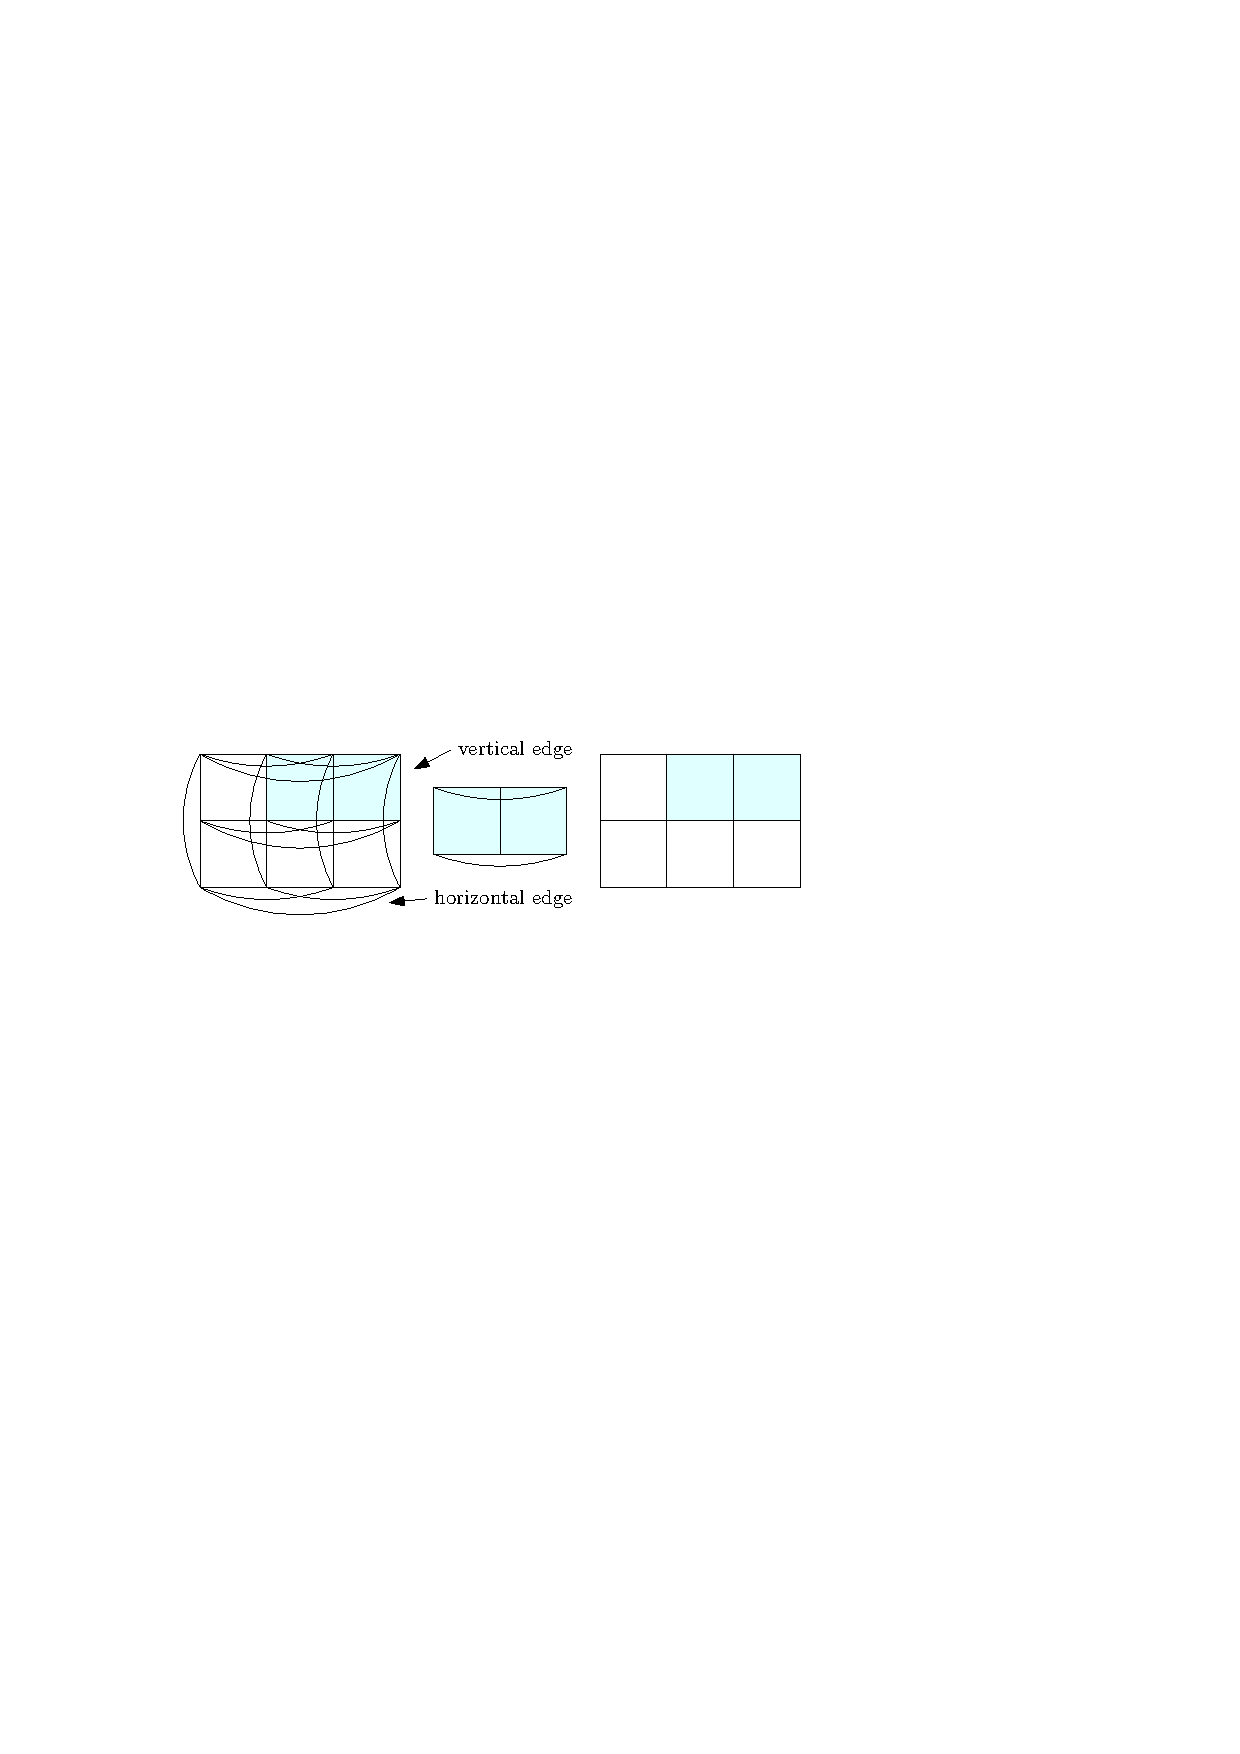
\includegraphics{uso_example.pdf}
  	\caption{\small The grid on the left is a $(4,3)$-grid (that means $4$ columns and $3$ rows) 
  	and a $(3,2)$-subgrid is shaded. The orientation on the right is a unique sink orientation of a $(3,2)$-grid.} 
  	\label{fig:examplegrid}
  \end{figure}



\subsubsection{Previous work.}

Unique sink orientations of grids, as presented in this paper,
are a graph-theoretic model for a specific class of linear programs~\cite{linepoint}.
Namely, assume that the feasible region of a given linear program is a
simple polytope of dimension $d$ that has exactly $d+2$ facets.
Every such \emph{$(d, d+2)$-polytope} is a product of two simplices and hence its graph $G$ is isomorphic to a grid~\cite{grid05}. 
Let $f : \RR^d \to \RR$ denote the objective function of the linear program.
Assuming general position, $f$ induces an orientation on $G$ such that for every oriented
edge $u \to v$ we have $f(u) > f(v)$ and the resulting digraph is a grid USO~\cite{grid05}.
Therefore, minimizing~$f$ on the polytope corresponds to finding the
unique sink of the grid USO $G$.

It is known that the above linear programming problem is equivalent to the \emph{One line and $n$ points} problem in the plane~\cite{linepoint,welzl2001entering}:
Given $n$ points in general position in the plane and one vertical line $\ell$, find the segment connecting two pairs of points that has the lowest intersection with the given line. 
We assume that $\ell$ contains none of the given points and that no two segments intersect on $\ell$.
\citet{linepoint} proved that the grid USO arising from an instance of the one line and $n$ points problem is a special grid orientation, called \emph{Holt-Klee} grid USO, which is a grid USO with a specific forbidden subgraph called the ``double twist'' depicted in Figure~\ref{fig:examplegrid} (right). In other words, each instance of the one line and $n$ points, and hence also each instance of a linear program on a $(d, d+2)$-polytope, corresponds to a Holt-Klee grid USO. 
However, the Holt-Klee condition is more general as there are grid USOs that satisfy it and  do not come from instances of the one line and $n$ points problem \cite{grid05}. 

An analysis of the \emph{Random Edge} simplex algorithm in the setting of one line and $n$ points provides a way to find the lower-most segment using $O(\log^2 n )$ pivot steps~\cite{linepoint}. 
An instance where this algorithm needs $\Omega(\log^2 n )$ many pivot steps is also provided. 
It can also be shown that geometry is not essential for Random Edge: Finding the sink of a Holt-Klee $(m,n)$-grid USOs it takes also $O(\log n\cdot\log m)$ vertex queries~\cite{grid05,falkthesis}. 

%for randomized \sinkalg in square Holt-Klee grid USOs using $O(\log^2 n)$ vertex queries~\cite{falkthesis}. 
%In addition, the Random Edge algorithm is generalized by \citet{grid05}, who prove that it also finds the sink of any %Holt-Klee $(m,n)$-grid USO using $O(\log n\cdot\log m)$ pivot steps with any starting vertex. 
%Finally, they argue that there are $2^{\Omega(n^2)}$ different Holt-Klee grid USOs.

\citet{grid08} study higher dimensional grid USOs (Cartesian products of $d$ complete graphs, each on at most $n$ vertices). 
%as general models that arise from solving a problem called PGLCP. \AT{We either say PGLCP is or we don't write PGLCP at all.} 
They provide a randomized product algorithm, which is similar to the one introduced in~\cite{SW} for cube USOs, and prove that for fixed dimension $d$ it uses polylogarithmic vertex queries in expectation. 
In particular, it finds the sink of any 2-dimensional grid USO using expected $O(\log n \cdot \log m)$ vertex queries which matches the performance of \sinkalgs in Holt-Klee grid USOs. Note, however, that a matching lower bound for the problem in the randomized setting remains elusive.
In the edge query model, again for fixed dimension, they describe a randomized \sinkalg that performs a linear number of queries.

Notice that that any algorithm that finds the sink of a grid USO using edge queries can be also applied to solve the following \emph{matrix USO optimization} problem: Find the global minimum of an injective real function defined on a two dimensional matrix USO, where a matrix is USO if each $2\times 2$ sub-matrix has a unique minimum. 
Therefore, the randomized algorithm from~\citet{grid08} solves the matrix USO optimization problem on a $m\times n$ matrix in $\Theta(m+n)$ expected time. However, no deterministic counterpart to this algorithm is known. 
Similar optimization problems on matrices have been studied with stronger conditions and have several applications in geometric problems~\cite{aggarwal1987geometric,demaine2005optimizing,galil1992dynamic,mityagin2003complexity}.

\subsubsection{Connection to LP-type problems.} \citet{grid08} hint that the problem of finding the sink of an $(m,n)$-grid USO can be naturally written as an \emph{LP-type problem}. An LP-type problem, originally defined by \citet{SharirW92}, is a pair $(S,w)$ where $S$ is a finite set called the \emph{constraints} and
$w:2^S \rightarrow \mathbb{R} \cup \{-\infty\}$ is a function subject to certain conditions: 
%\citet{DBLP:journals/dam/GartnerMRS08} looked also at the connection with the more general setting of \emph{violator spaces}.
(1) Monotonicity: for every two sets $A \subseteq B \subseteq S$, we have $w(A) \leq w(B) $ and
(2) Locality: for every two sets $A \subseteq B \subseteq S$ and every constraint $h \in S$, if $w(A) = w(B) = w(A\cup \{h\})$ then $w(A) = w(B \cup \{h\})$.
A set $B \subseteq S$ is called a \emph{basis} if every proper subset
of $B$ has a smaller value of $w$ than $B$ itself. The \emph{combinatorial dimension} of an LP-type problem 
is the maximum cardinality of a basis
(for more information on LP-type problems refer to \cite{MatousekSW96}). 

%\citet{grid08} hint that the problem of finding the sink of an $(m,n)$-grid USO can be naturally written as an LP-type problem $(S,w)$ of combinatorial dimension~2 (\citet{DBLP:journals/dam/GartnerMRS08} looked also at the connection with the more general setting of \emph{violator spaces}). 
To write a grid USO as an LP-type problem, we let the set of constraints $S$ be the set of rows and columns and therefore $|S| = m + n$. As any grid USO is acyclic (see Section~\ref{section:grid_uso_properties}), there is a topological ordering of its vertices. 
The function $w$ then takes a subset of the rows and columns defining a subgrid and maps it to the rank of its sink in the topological ordering. 
If the subset of $S$ consists only of rows or columns, its value under $w$ is~$-\infty$. 
This definition satisfies both monotonicity and locality yielding an LP-type problem.
Moreover, a basis is simply a vertex defined by two constraints, one row and one column.
Finding the sink of the grid then corresponds to finding a basis of $(S,w)$ with the highest value.
%The \emph{violator set} of a vertex $v$ is the set of constraints representing the rows and columns to which $v$ has outgoing edges. 

There are linear-time randomized algorithms for LP-type problems~\cite{MatousekSW96} that, by the above construction, yield \sinkalgs using linear number of edge queries. 
While there exist deterministic algorithms with matching asymptotic performance to solve LP-type problems \cite{chan16,ChazelleM96}, they make an extra assumption on the problem 
(see Computational assumption 2 in \cite{ChazelleM96}). 
A necessary requirement they make is that a specific set system has constant VC-dimension which does not hold for the LP-type problem in grid USOs described above (refer to~\cite{matouvsek2002lectures} for further information on set systems and VC-dimension). More specifically, for each vertex $v$ in the grid, let $R_v\subset S$ be the set of rows and columns to which $v$ has an outgoing edge. 
The \emph{violator set system} $(S, \mathcal R)$ must have constant VC-dimension for the above deterministic algorithms to work, where $\mathcal R = \{R_v : v\text{ is a vertex of the grid}\}$. 
Since this set system has unbounded VC-dimension for general grid USOs, as illustrated in Figure~\ref{fig:shatteredgrid}, these deterministic algorithms are less efficient than exploring the entire grid exhaustively. 
Therefore, it is open whether there exist deterministic \sinkalgs that use less than a quadratic number of queries. 
%In particular, it is not known if \emph{any} LP-type problem can be deterministically solved in linear~time. 

Curiously, if the grid USO satisfies the Holt-Klee condition, then its violator set system has VC-dimension at most 2.
%While the above deterministic algorithms for LP-type problems are not efficient for general grid USOs, the addition of the Holt-Klee condition yields efficient \sinkalgs:
This is a consequence of the fact that every Holt-Klee grid USO is induced by a red-blue arrangement of pseudo-lines \cite{grid05,falkthesis}, and such an arrangement always has VC-dimension at most 2.
%In turn, this can be thought of as the dual of the combinatorial version of the one line and $n$ points configuration.
Despite that, the results of \citet{ChazelleM96} still do not directly imply a deterministic algorithm using $O(m+n)$ edge queries for finding the sink of a Holt-Klee $(m,n)$-grid USO because of the further requirements in Computational assumption 2 of \citet{ChazelleM96}.

%Therefore, we can deterministically find the sink of Holt-Klee grid USOs using only a linear number of queries by reducing it to an LP-type problem~\cite{chan16,ChazelleM96}.


\begin{figure}[h!] 
  	\centering
  	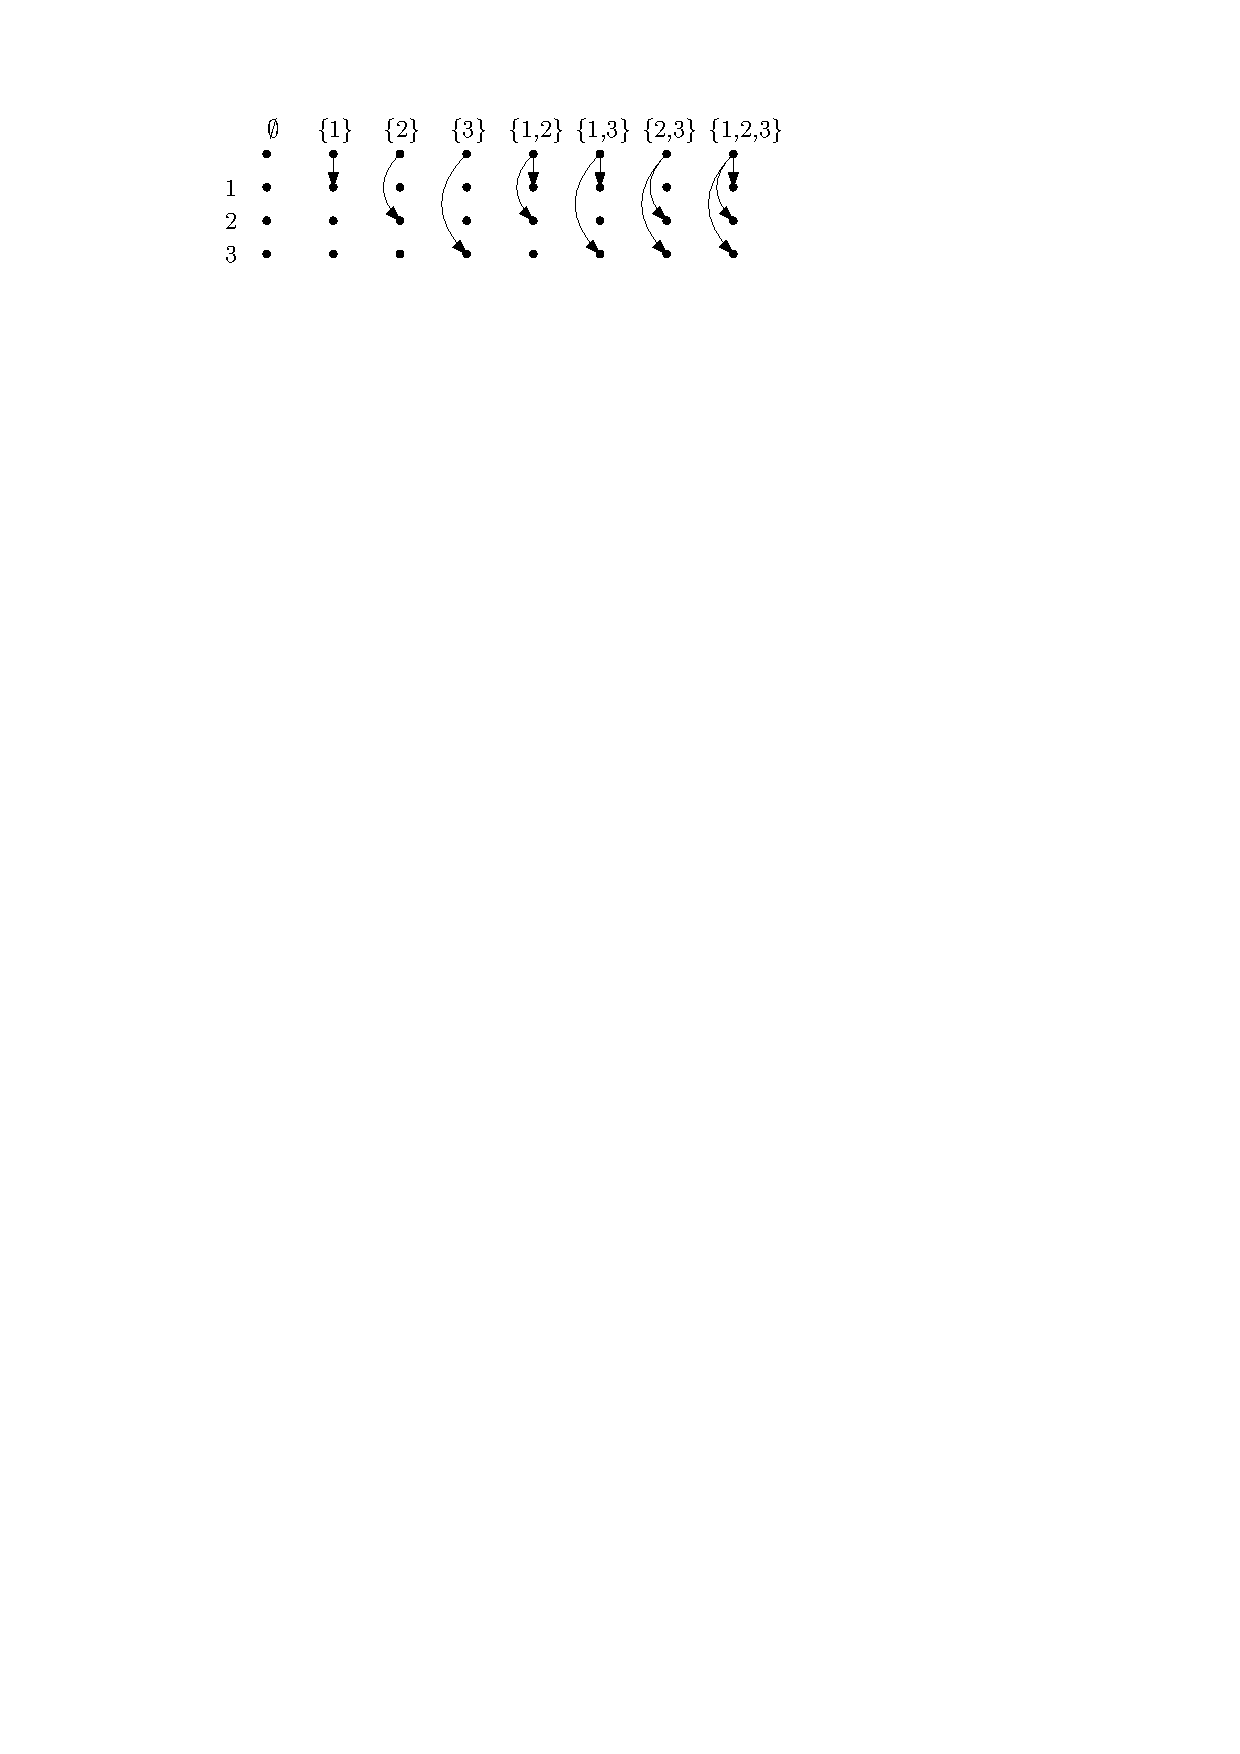
\includegraphics{shatteredgrid.pdf}
  	\caption{\small We display an $(n,\log n + 1)$-grid USO whose violator set system has VC dimension at least $\log n$. 
	  The columns are labeled with the subsets of the powerset of $\{1,2,3\}$. On the top, unlabeled, row we have a vertex whose 
	  vertical outgoing edges correspond to the set on the label of the column. Incoming edges are not depicted for these vertices. Also none 
	  of the edges of the grid that are not incident to one of the vertices of the top row. All the horizontal edges are uniformly oriented to the left.
	  This orientation can be easily extended to a grid USO.} 
  	\label{fig:shatteredgrid}
  \end{figure}
  


%Namely, they require that the set system induced on $S$ by the family of violator sets of each of the vertices has constant VC-dimension (refer to~\cite{matouvsek2002lectures} for further information on VC-dimension).

%The deterministic algorithm for LP-type problems by \citet{DBLP:journals/jal/ChazelleM96} 

%There is a natural way to write a $(m,n)$-grid USO as an LP-type problem of combinatorial dimension 2. There are randomized algorithms for LP-type problems that imply $\Theta(m+n)$ edge queries for ($m,n$)-grid USOs in expectation. It was hinted by \citet{grid08} that it might be possible to apply the deterministic algorithms for LP-type problems \cite{DBLP:journals/jal/ChazelleM96} also for $(m,n)$-grid USOs. However, these deterministic algorithms assume an extra condition (called Computational assumption 2 in \cite{DBLP:journals/jal/ChazelleM96}) 

\subsubsection{Our results.}

While randomized algorithms to find the sink of a grid USO have been previously studied~\cite{grid05,linepoint,grid08,falkthesis}, 
to the best of our knowledge no non-trivial deterministic algorithm was known prior to this work. 
We present the first deterministic algorithms that find the sink of an $(m,n)$-grid USO using $O((m+n)\log (m+n))$ vertex queries
and 
%we present the first non-trivial deterministic algorithm that finds the sink of an $(m, n)$-grid USO using 
$O((m+n)^{\log_47})$ edge queries respectively.
Both query models exhibit a lower bound of $\Omega(m+n)$ queries.

Since a single vertex query reveals the orientation of a linear number of edges, one would expect the minimum number of  oracle queries required to find the sink to be different in the edge and the vertex query models.
Indeed, as shown ~\citet{grid08} this is true for randomized algorithms where there is an exponential gap ($O(\log m\cdot \log n)$ vertex queries and $\Theta(m+n)$ edge queries suffice to find the sink of a grid USO).
However, in the deterministic setting, it is still unclear whether a gap exists.

Additionally, recall that an algorithm that finds the sink of a grid USO in the edge query model can be used to solve the matrix USO optimization problem. 
Therefore, our algorithm in the edge query model provides a way to deterministically find the minimum of an $m\times n$ matrix USO by querying for the value of only $O((m+n)^{\log_4 7})$ entries of the matrix. 

\subsubsection{Outline.}
%To guide the reader, we give a rough sketch of the algorithms presented in this paper.
%The main idea behind our algorithms is to partition the grid into a constant number of subgrids. 
%Then, by recursively finding the sink of a ``few'' of these subgrids, we are able to infer global %information and discard some of the remaining subgrids, i.e., we guarantee that they do not contain the sink. 
%In this way, there are portions of the grid where no oracle query is performed which leads to algorithms that require a sub-quadratic number of oracle queries.

In Section~\ref{section:grid_uso_properties} we state basic facts for grids that were already known from previous work. Subsequently, we define a way to partition the grid into subgrids and discuss the properties of this partition. The notion of induced grid USOs becomes relevant and we describe Lemma~\ref{lemma:USO-Lemma} which is crucial for our algorithms.

In Section~\ref{section:the_sink_finding_algorithm} we focus on the vertex query model and prove a our main result: Theorem~\ref{theorem:Sink algorithm}. Finally, in Section~\ref{section:The edge oracle model} we briefly discuss the edge query model and give the relevant algorithm in Theorem~\ref{thm:timeEdge}.

%and improve upon the above algorithm by using the following idea: Spend a linear number of vertex queries prior to the partition to discard an $(n/2, n/2)$-subgrid that contains one quarter of the total number of vertices. 
%The removal of such a subgrid leaves us with a graph that can be partitioned into three $(n/2, n/2)$-subgrids. 
%We then show how to find the sink by recursively solving only two of them and disregarding the third one. In this way, we obtain a recurrence of the form $T(n) = 2 T(n/2) + O(n)$ which solves to $O(n \log n)$. 
%That is, we obtain a deterministic algorithm that finds the sink of an $(n, n)$-grid using $O(n \log n)$ vertex queries. \AT{I leave the outline section unedited. Let us first decide why and when to talk about square grids. Also look for this at the beginning of Section 3, Sink-finding algorithm.}

%To fix ideas, imagine splitting an $(m,n)$-grid into four $(m/2, n/2)$-subgrids. In Section~\ref{lemma:USO-Lemma} we show how to partition the grid into subgrids


%In Section~\ref{lemma:USO-Lemma} we show how to find the global sink of this grid by recursively solving only three of the four $(n/2, n/2)$-subgrids while disregarding the last one. \AT{What is this? Is it still in?}
%We obtain then a recurrence of the form $T(n) = 3 T(n/2)$ which solves to $T(n) = O(n^{\log_2 3})$.
%More involved arguments allow us to split the grid into 16 subgrids and find the sink by solving only 7 of them which leads to a deterministic algorithm using $O(n^{\log_4 7})$ oracle queries.



%To discard the $(n/2, n/2)$-subgrid used in the first part of this algorithm, we focus on finding a vertex $v$ with ``large'' indegree. 
%However, we want the incoming edges of $v$ to be evenly distributed among its horizontal and vertical edges. Using the properties of the grid USO, we are able to show that such a vertex $v$ will be the sink of a large subgrid, namely the smallest subgrid that contains $v$ and each vertex that has an outgoing edge to $v$.
%If the indegree of $v$ is sufficiently large, then this subgrid having $v$ as its sink will contain a quarter of the vertices of the $(n,n)$-grid fulfilling the requirements of our $O(n \log n)$ algorithm.

%While the first $O(n^{\log_4 7})$ algorithm works in both the edge- and the vertex-query model, we have not been able to extended the second and more efficient algorithm to the edge-query model.


\section{Grid USO Properties}\label{section:grid_uso_properties}


%The set of \emph{indices} of an $(m,n)$-grid is $[m]\cup [n]$.


%\begin{lemma}[Product construction]
% Let $G$ be an $X\times Y$-grid USO for some sets $X$ and $Y$ and let $A \subset 2^X$ and $B \subset 2^Y$ be partitions of $X$ and $Y$, respectively. Let $H$ be an $A\times B$-grid. \JN{See Malte's 4$\times$4 lower bound for a possible way to define this.}
%\end{lemma}
Recall that an induced subgraph of a grid is called a \emph{subgrid} if it is itself a grid.
The subgrids of an $(m,n)$-grid are exactly those induced subgraphs whose vertex set is a
Cartesian product $I \times J$, for some $I \subseteq [m]$ and $J \subseteq [n]$. We call the corresponding subgrid an $I\times J$-subgrid.
If the original grid is oriented, the subgrids inherited an orientation. 

Our algorithms rely on two basic properties of grid USOs.
First, \citet{grid08} have shown that every $(m,n)$-grid USO is \emph{acyclic}. 
The second ingredient is a partitioning strategy which we describe subsequently.

\subsubsection{Induced USOs.}

For our algorithms we want to partition the grid into subgrids.
Such a partition into subgrids forms itself a grid in a natural way,
which inherits a unique sink orientation from the original grid USO; see Figure~\ref{fig:example_induced_orientation} for an illustration.

  \begin{figure}[htbp] 
  	\centering
  	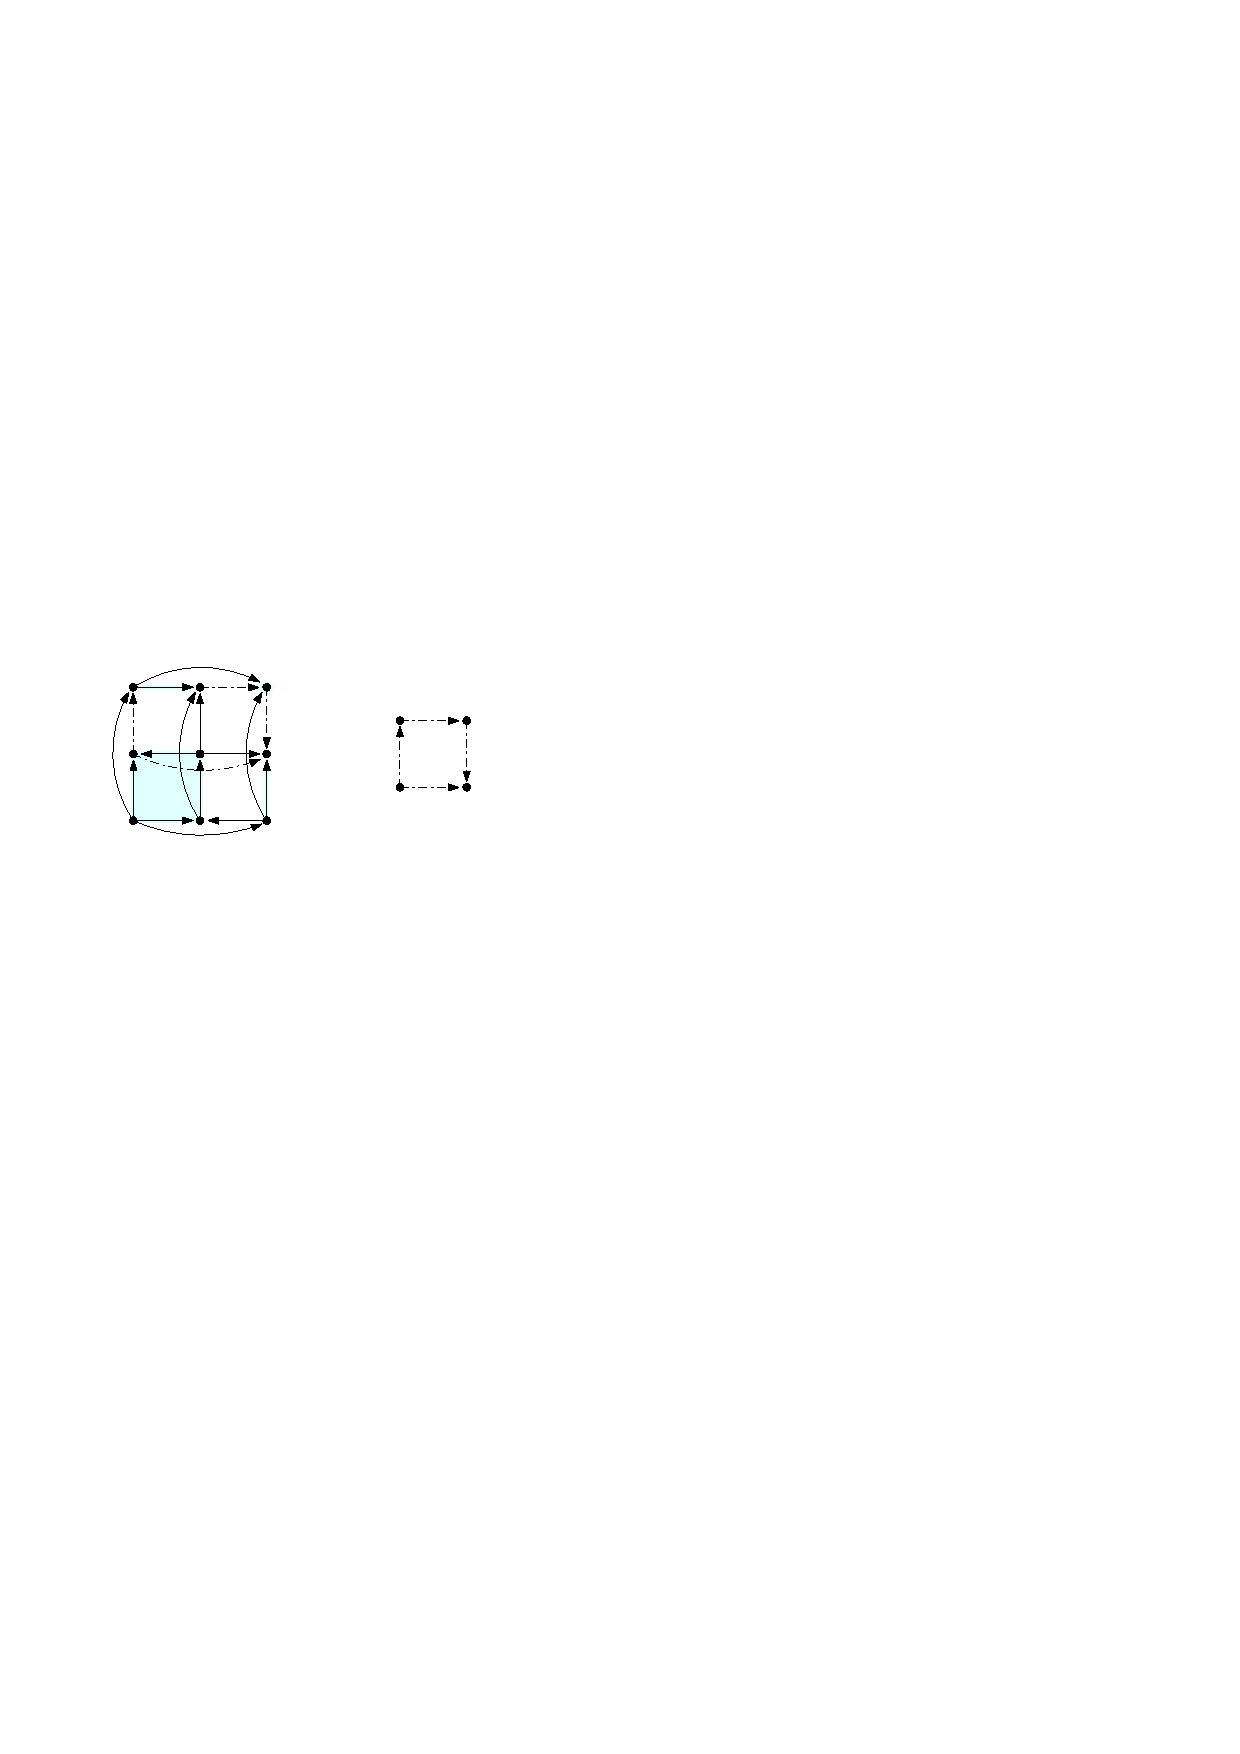
\includegraphics[scale=1]{induced_orientation_ex.pdf}
  	\caption{\small On the left side of the figure there is a $(3,3)$-grid USO whose $X$-coordinates and $Y$-coordinates have been partitioned into 2 parts of cardinalities two and one. The induced $(2,2)$-grid USO with respect to these blocks is shown on the right; the edges contributing to the induced orientation are also shown in the original grid.} 
  	\label{fig:example_induced_orientation}
  \end{figure}

Formally, let $G$ be an $(m,n)$-grid USO,
and let $\A = \{A_1,\ldots,A_k\}$ and $\B = \{B_1\ldots, B_l\}$ be partitions of $[m]$ and $[n]$, respectively.
Let $H$ be a $(k,l)$-grid whose vertex $(i,j)$ we identify with the $A_i \times B_j$-subgrid of $G$ for every $1\leq i \leq k$ and for every $1 \leq j \leq l$. 
We define an orientation on $H$ so that the edge between two adjacent vertices $x$ and $y$ of $H$ is oriented towards $y$ if the sink of $x$ has at least one outgoing edge to a vertex of $y$ in the original grid $G$. 
This orientation is well defined: If the sink of $y$ also had an edge towards some vertex of $x$, there would be a cycle in $G$. 
Furthermore, there is always at least one such outgoing edge from one of the sinks as otherwise an appropriately chosen subgrid of $G$ would have two sinks. 
We say that this orientation is \emph{induced} on $H$ by $G$ and $H$ is called the \emph{\abpart}. 
The following result shows that the orientation induced on $H$ by $G$ is also a unique sink orientation. 
A similar result was proved by G\"artner et al.~\cite{grid08} in higher dimensional grid USOs.

%Let $H = K_\A \times K_\B$ be the \emph{$\A$-$\B$-partition grid} of $G$.


%For every vertex $x = (A,B)$ of $H$, where $A\in \A$ and $B \in \B$, let $G(x)$
%denote the $A \times B$-subgrid of $G$. 

\begin{lemma}[USO-Lemma]\label{lemma:USO-Lemma}
Let $G$ be an $(m,n)$-grid USO,
and let $\A$ and $\B$ be partitions of $[m]$ and $[n]$, respectively.
The orientation of the $\A$-$\B$-partition grid $H$ induced by $G$ is a unique sink orientation.
Moreover, the sink of $H$ is the subgrid of $G$ that contains the sink of $G$.
\end{lemma}
%\begin{theorem}
%\label{thm:the_sink_of_the_sink_of_the_induced_orientation_is_the_global_sink}

%Let $G$ be an $(m,n)$-grid USO,
%and let $\A$ and $\B$ be partitions of $[m]$ and $[n]$, respectively. Let $A\in \A$ and $B \in \B$.
%If the $A\times B$-subgrid is the sink of the $\A$-$\B$-partition grid $H$, then the sink of the $A\times B$-subgrid is the sink of $G$.
%\end{theorem}

\section{The Vertex Oracle Model}
\label{section:The vertex oracle model}

Recall that in the vertex query model a grid USO is given by a \emph{vertex oracle} that for a queried vertex reveals the orientations of the edges adjacent to the vertex. 
An adversary argument can be used to show that any deterministic algorithm needs $m+n-1$ vertex queries in the worst case to find the sink of an $(m, n)$-grid USO.
Our main result is Theorem~\ref{theorem:Sink algorithm} which describes a deterministic algorithm that needs $O((n + m) \log (n + m))$ vertex queries. 

\subsubsection{The Sink-finding Algorithm.}
\label{section:the_sink_finding_algorithm}

Before explaining the algorithm we introduce some notation. We define a reflexive partial order on the vertices of a grid USO $G$ as follows. 
For any two vertices $v,w \in G$ we say that $w \succeq v$ if there is a directed path from $w$ to $v$ within the grid $G$ (or if $w = v$). 
In words, we say that $w$ is \emph{larger} than $v$ (or $v$ is \emph{smaller} than $w$).
Because grid USOs are acyclic, this partial order is well defined.
Moreover, the sink of the grid USO is the unique minimal vertex with respect to this ordering. 

For a set of vertices $V$ in a grid USO $G$ let $\join(V$) be the set of vertices of the grid to which there is a path from all vertices in $V$.  More formally $\join(V) = \{w \in G \: | \: v \succeq w \:\: \forall v \in V \}$. Note that if $s$ is the sink of the subgrid containing two vertices $v$ and $w$, then $s \in \join(\{v,w\})$. Therefore, given some set of vertices $V$, we can compute a $w \in \join(V)$ with $O(|V|)$ vertex queries.

%Note that two vertices may not be $\succeq$-comparable in the smallest subgrid containing them. 
%There could still be a path between the two vertices. 
%Thus\JN{after the transitive closure they might still be incomparable}, we consider the transitive closure of this relation and say that a vertex $w$ is \emph{larger} than $v$ (or $v$ is smaller than $w$) if there is a sequence $w = v_1, v_2, \ldots, v_k = v$ of $G$ such that $v_i \succeq v_{i+1}$, for each $1\leq i\leq k-1$.

In an ($m,n$)-grid USO $G$, the \emph{\indegree} of a vertex $v \in G$ is an ordered pair $[a_v, b_v] \in \{0,1,\ldots,m-1\}\times \{0,1,\ldots,n-1\}$ where $a_v$ and $b_v$ specify the number of incoming horizontal  and vertical edges of $v$, respectively.
We say that a vertex $v$ with \indegree $[a_v, b_v]$ is a \emph{$(k, t)$-vertex} if $a_v\geq k-1$ while $b_v\geq t-1$.

Consider the following algorithmic approach to finding the sink of an ($m$,$n$)-grid USO deterministically. 
Assume that we are able to find in $O(m+n)$ time a $(\frac{m}{2}, \frac{n}{2})$-vertex $v$.
We could then partition the grid into 4 equally sized square subgrids so that $v$ is the sink of one of them.
The next step would be to find the sink of the block antipodal to the block containing $v$ in the (2,2)-grid induced by this partition. 
By Lemma~\ref{lemma:USO-Lemma} we could thereafter discard one subgrid out of consideration and possibly still find the sink of one subgrid.
If one finds the sinks of the subgrids recursively, one would get the recursion
\begin{align*}
 T(m,n) = 2T\left(\frac{m}{2},\frac{n}{2}\right) + O(m+n)
\end{align*}
where $T(m,n)$ is the number of vertex queries needed by this algorithm to find the sink of an $(m,n)$-grid. This recurrence solves to \mbox{$T(m,n) = O((m+n)\log (m+n))$}. 

The main part of the algorithm description is to obtain an $(\frac{m}{2}, \frac{n}{2})$-vertex in linear time.
For ease of presentation, we prove Lemmas~\ref{lem:diagonal_lemma} and \ref{lem:seed_lemma_for_square_matrices} for the square $(n, n)$-grid. From those, 
we obtain Corollary~\ref{corollary: n/4 indegree}, which we state here without proof.  The latter establishes the computation of a 
$(\frac{m}{8}, \frac{n}{8})$-vertex in linear time. Using it as a black box, we manage to get a $(\frac{m}{2}, \frac{n}{2})$-vertex with only linearly 
many more queries in Lemma~\ref{lemma:Climbing lemma} and Corollary~\ref{corollary: (m/2,n/2) indegree}.

\begin{lemma}
\label{lem:diagonal_lemma}
Let $D = \{v_1,\ldots,v_n\}$ be the set of diagonal vertices of an $(n,n)$-grid USO so that $v_i = (i,i)$. After sorting the vertices with respect to their indegree the $j$-th vertex has at least $j-1$ incoming edges.
\end{lemma}

\begin{proof}
Note that to prove the claim it is enough to show that some ordering of~$D$ has the property that the $j$-th vertex has at least $j-1$ vertices because then also the ordering with respect to indegree satisfies the same property. 

Rename the coordinates such that for all $1 \leq i < j\leq n$ either $v_i \succeq v_j$ or $v_i$ and $v_j$ are incomparable. 
This defines a linear extension of the partial order $\succeq$ and we claim that $v_j$ has at least $j-1$ incoming edges for every $j = 1, \ldots, n$. 
To see this fix some $v_j$ and consider the $(2,2)$-subgrid $H_{i,j}$ containing both $v_i$ and $v_j$ for some $1\leq i < j$. 
Because $H_{i,j}$ is a USO and since $v_i \succeq v_j$ (or $v_i$ and $v_j$ are incomparable), we know that $H_{i,j}$ contains no path from $v_j$ to $v_i$. 
Therefore, $v_j$ cannot be the source of $H_{i,j}$  which implies that $v_j$ has at least one incoming edge in $H_{i,j}$. 
Since the edges in $H_{i,j}$ are disjoint from those of $H_{i',j}$ for $1\leq i < i' < j$, 
we know that $v_j$ has an incoming edge for each $1\leq i< j$, i.e., $v_j$ has at least $j-1$ incoming edges. 
%To prove our claim we first show that after querying the diagonal in the first phase, and after sorting and renaming the vertices, $D$ has the property that $v_i$ has at least $i-1$ incoming edges.
%To prove the claim, observe that if some ordering has the property, then the ordering with respect to the number of incoming edges satisfies the property as well. \JN{To Luis You commented before that you didn't see the argument. I modified it so hopefully now it works.}
%The existence of such an ordering follows by considering any linear extension of $\succeq$ restricted on $D$. 
%Indeed, if $D$ was ordered so that $v_i \not\preceq v_j$ for all $i\leq j$, then consider the $(2,2)$-subgrids containing two diagonal vertices: For every $i < j$ the $(2,2)$-subgrid containing $v_i$ and $v_j$ has at least one edge oriented towards $v_j$ because otherwise this would contradict the assumption on having a linear extension. 
%This proves our first claim.
 \qed
\end{proof}



\begin{lemma}
\label{lem:seed_lemma_for_square_matrices}
 Given an $(n, n)$-grid USO we can find an $(\frac{n}{4}, \frac{n}{4})$-vertex using $O(n)$ vertex queries.
\end{lemma}

\begin{proof}
The algorithm we describe queries a linear number of vertices of the grid before finding a vertex with the required \indegree. 
After explaining the algorithm, we prove its correctness.

%The algorithm works as follows. 
In the first phase, query the diagonal vertices $D = \{v_1,\ldots, v_n\}$ where $v_i = (i,i)$.
If one of the vertices in $D$ has the required \indegree, we are done. 
If not, sort and rename the vertices of $D$ such that for $i < j$ vertex $v_i$ has at most as many incoming edges as $v_j$. 

In the second phase, let $V = \{v_{\lceil \frac{n}{2} \rceil},\ldots,v_n\} \subseteq D$.
Label the vertices in $V$ as either \emph{horizontal}  or \emph{vertical}, depending on whether the majority of incoming edges for the corresponding vertex are horizontal  or vertical, respectively. 
Assume without loss of generality that there are more vertical vertices in $V$; otherwise change the role of the coordinates. 
Let $V' \subseteq V$ be the set of all vertical vertices in $V$ and notice that $|V'| \geq |V|/2$.
Then, find some $v \in \join(V')$ by using at most $O(V')$ additional queries and note that $v' \succeq v$ for every $v' \in V'$.

Let $I'$ be the set of indices containing the first coordinate of each vertex in~$V'$. 
Assume that $v = (x_v, y_v)$ and let $W = I'\times \{y_v\}$ be a subset of vertices in the same row as $v$ with $|W| = |V'|\geq |V|/2$.
To conclude, the algorithm queries each vertex in $W$.
It is clear from the description above that the number of vertices queried so far is $O(n)$. 
We claim that one of the queried vertices will have the required \indegree.

Because of the renaming after the first phase and due to Lemma~\ref{lem:diagonal_lemma} we know that $v_i$ has at least $i-1$ incoming edges. 
Therefore, by the definition of $V$, we know that each vertex of $V'\subseteq V$ has at least $\lceil \frac{n}{2} \rceil - 1$ incoming edges.
Moreover, each vertex in $V'$ has at least $(\lceil \frac{n}{2}\rceil-1)/2$ incoming vertical edges and $|V'| \geq \frac{n-\lceil \frac{n}{2}\rceil + 1}{2} \geq \frac{n}{4}$. 

Let $v^*$ be the sink of $W$ obtained after querying each vertex in this set (including $v$). Let $[a,b]$ be the \indegree of $v^*$. We claim that $a, b \geq \frac{n}{4} - 1$. 
Indeed, because $v^*$ is smaller than each other vertex in $W$, we know that $$a \geq |W|-1 = |V'|-1 = \frac{n-\lceil \frac{n}{2}\rceil + 1}{2} - 1 \geq \frac{n}{4} - 1.$$


%If $v = v^*$, then since $v\in V'$, we know that $b\geq \frac{\lceil \frac{n}{2}\rceil-1}{2}\geq \frac{n}{4} - 1$. \AT{Why is $v \in V^*$ now?}
Furthermore, there is a vertex $v' \in V'$ that is in the same column as $v^*$. Due to the \join operation there is a path from $v'$ to $v$ and further to $v^*$. 
If $v'=v^*$ then the we know already that $v^*$ has at least $\frac{n}{4} - 1$ incoming edges vertically.
Otherwise,  the edge between $v'$ and $v^*$ is oriented towards $v^*$ and $v^*$ has more incoming vertical edges than $v'$, because of acyclicity. Therefore we establish that $b \geq \frac{\lceil \frac{n}{2}\rceil-1}{2} + 1 \geq \frac{n}{4} \geq \frac{n}{4} - 1$ which shows that $v^*$ is an $(\frac{n}{4}, \frac{n}{4})$-vertex. \qed

%\begin{figure}[htbp] 
%\centering
%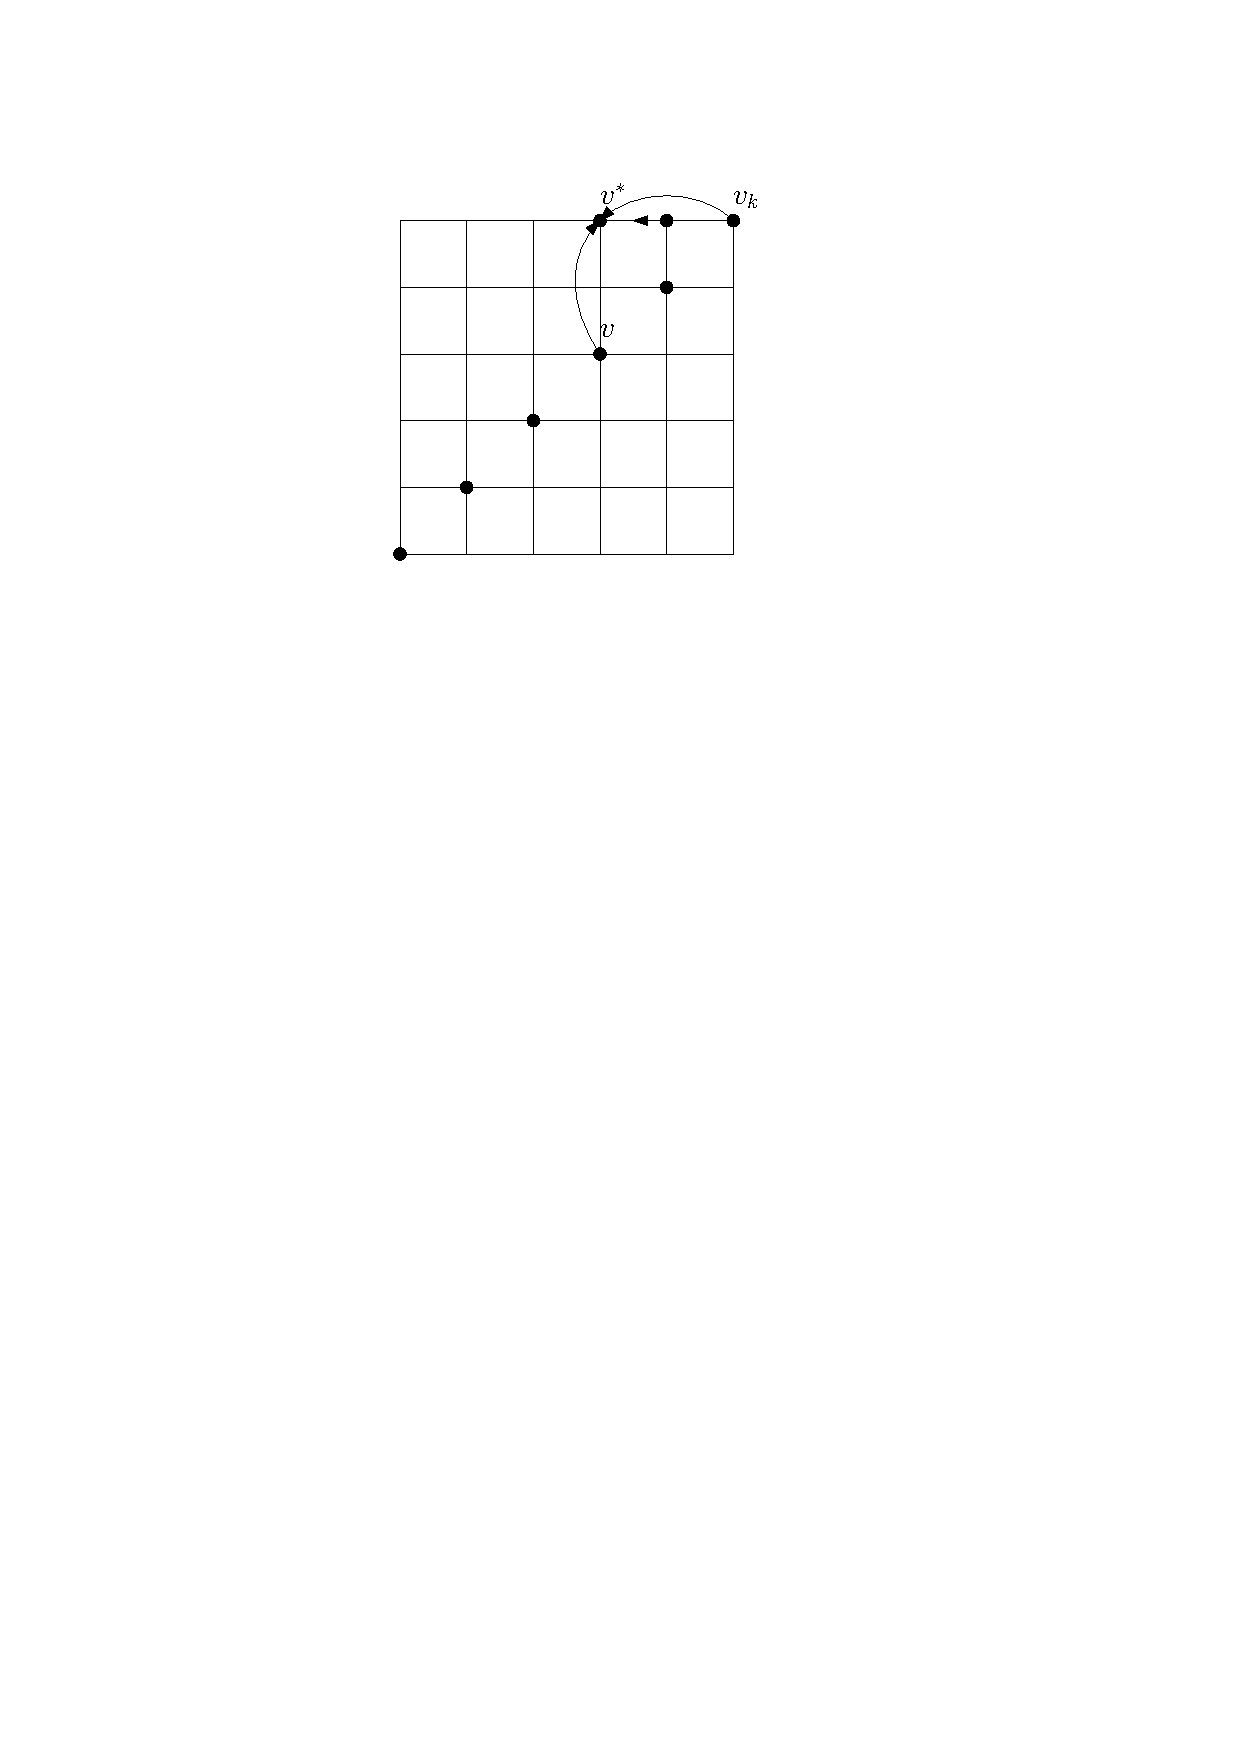
\includegraphics[scale=0.7]{seedlemma_fig1.pdf}
%\caption{In this figure only a subset of the edges of the grid appears. The vertices that are marked with discs are the ones evaluated.} 
%\label{fig:seedlem1}
%\end{figure}

 %If we can show that there is an edge from $w$ to $v^*$, then by acyclicity $v^*$ has at least one more incoming vertical edge as compared to $w$, therefore establishing that $b \geq \frac{\lceil \frac{n}{2}\rceil-1}{2} + 1 \geq \frac{n}{4} \geq \frac{n}{4} - 1$ and showing that$v^*$ is an $(\frac{n}{4}, \frac{n}{4})$-vertex. 
   
   %Because $v$ is a minimal vertex in $V'$, either $w\succeq v$, or $v$ and $w$ are incomparable. 
   %To show that there is an edge from $w$ to $v^*$ we study these two cases: 
   %\MM{If I'm following this correctly, then the case distinction is
   %unnecessary. An edge $v^* \to w$ would immediately contradict $v
   %\not\succeq w$.}
   %If $w \succeq v$, then because $v \succeq v^*$ we have due to transitivity that $w \succeq v^*$. 
  %Otherwise, $w$ and $v$ are incomparable. In this case, since $v^*$ is smaller than $v$, we know %that the edge connecting $v$ and $v^*$ is  oriented towards $v^*$. 
  %Therefore, the only possibility for $v$ and $w$ to be incomparable is that there is an edge from $w$ to $v^*$. 
  %We give illustrations of the two cases in Figure~\ref{fig:seedlem2}. 
  %Thus regardless of the case, there is an edge from $w$ to $v^*$ which concludes the proof. \qed  
%\begin{figure}[htbp] 
%    \centering
%    \begin{subfigure}[b]{0.4\textwidth}
%        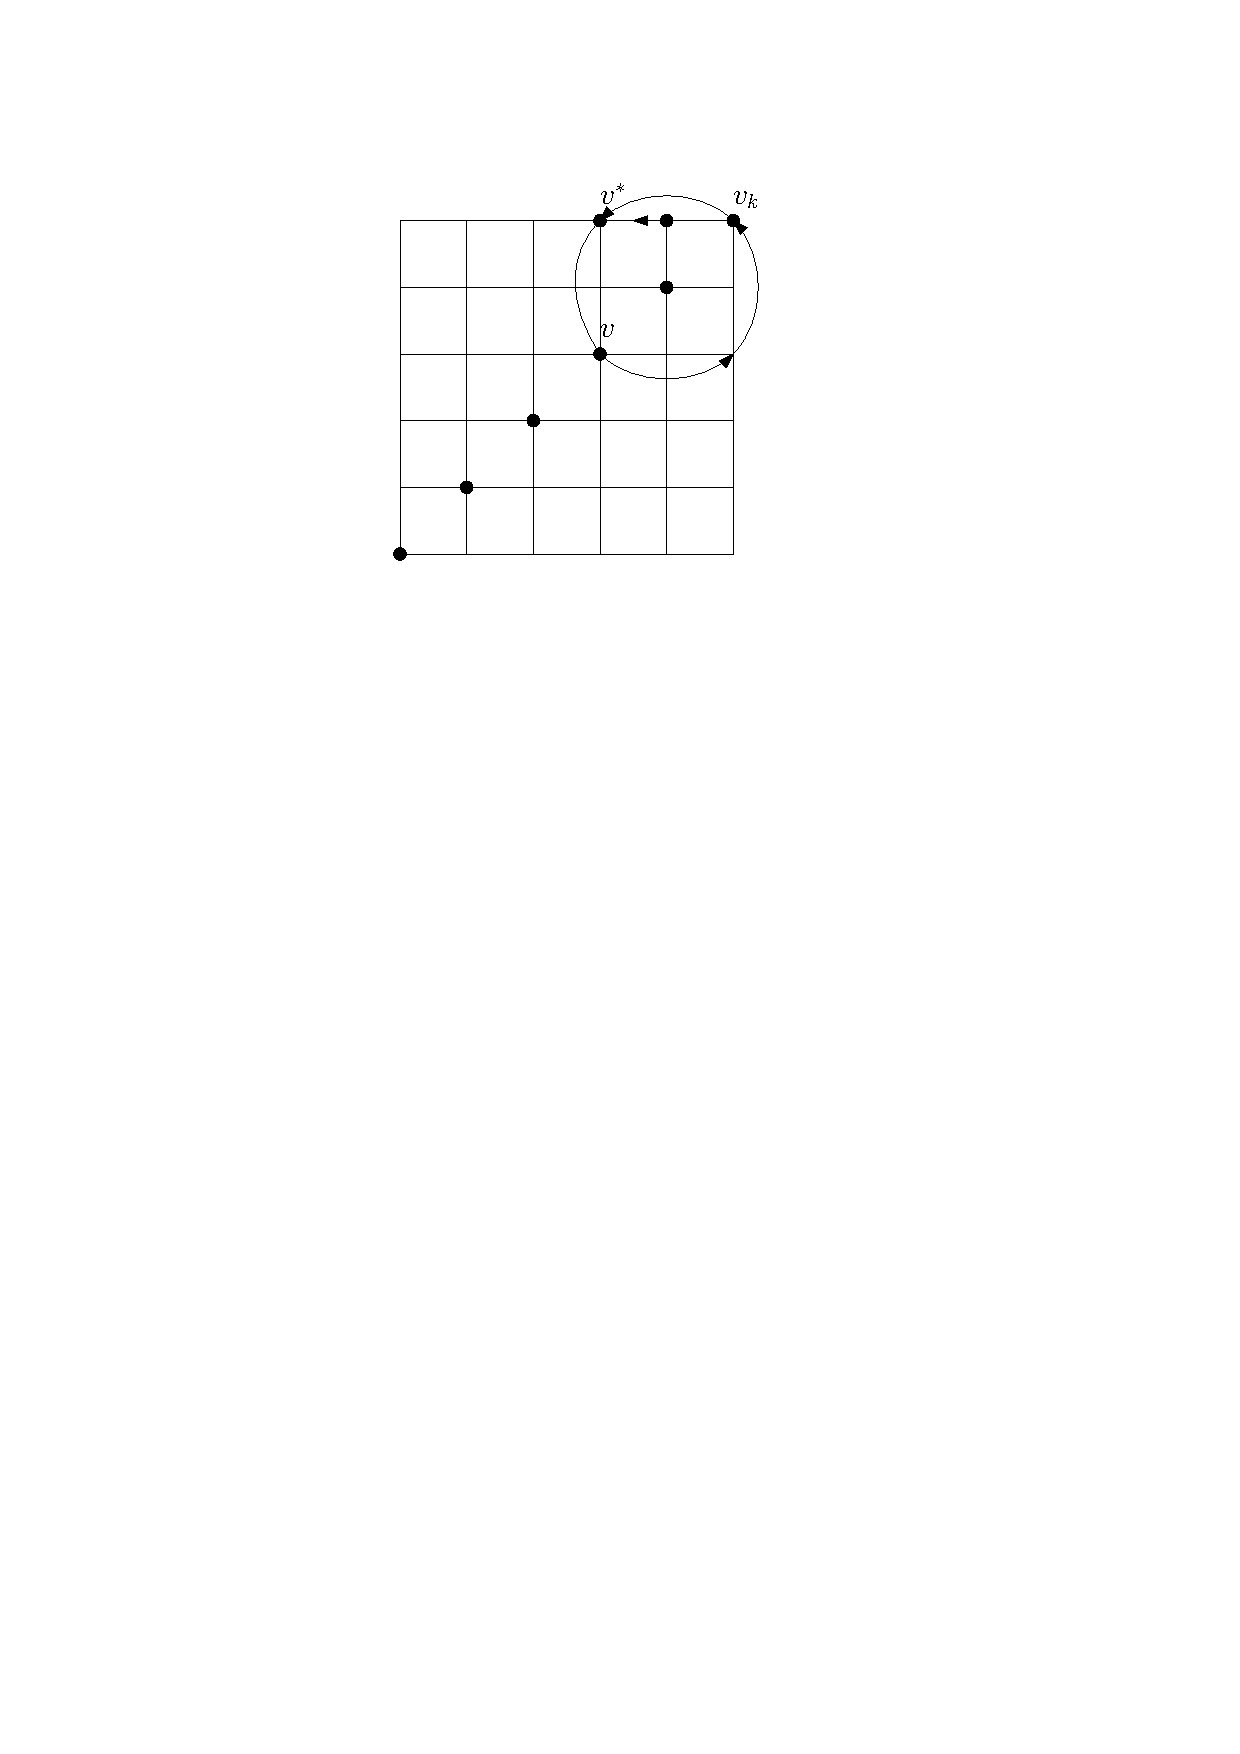
\includegraphics[scale = 0.7]{seedlemma_fig2_cas1.pdf}
%        \caption{$w \succeq v$}
%    \end{subfigure}
%    \qquad \qquad
%    \begin{subfigure}[b]{0.4\textwidth}
%        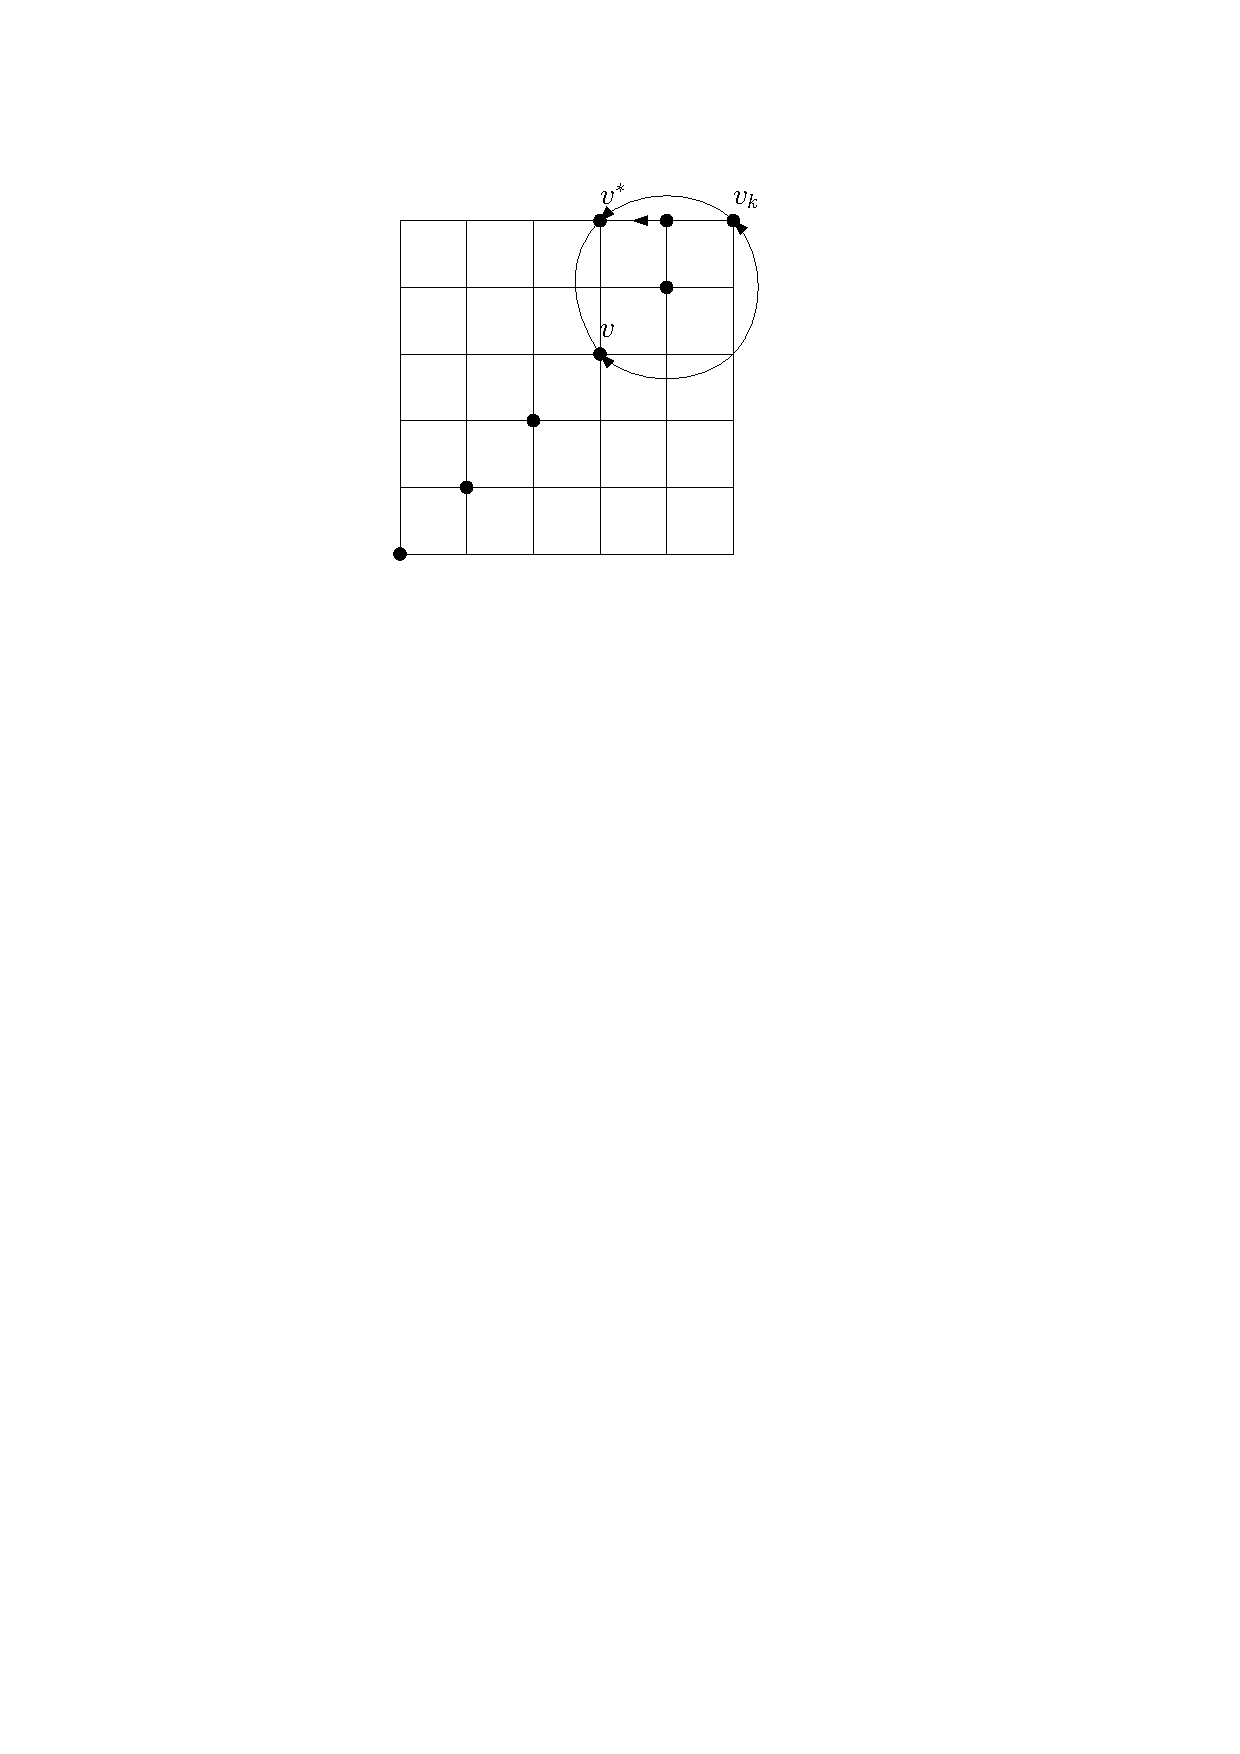
\includegraphics[scale = 0.7]{seedlemma_fig2_cas2.pdf}
%        \caption{$v$ and $w$ are incomparable}
%    \end{subfigure}
%    \caption{Illustrations of the two cases. }
%    \label{fig:seedlem2}
%\end{figure}
\end{proof}

The following corollary extends the previous lemma to non-square grids.

\begin{corollary}\label{corollary: n/4 indegree}
  Given an $(m,n)$-grid USO $G$, we can find a vertex with \indegree $[a,b]$ with $a \geq \frac{m}{8} - 1$ and  $b \geq \frac{n}{8} - 1$ using $O(m+n)$ vertex queries.
\end{corollary} 


%if every induced directed subgraph that is attained by fixing or limiting the range of some coordinates of the vertices has a unique sink. More specifically, we require this property to hold for subgraphs that are attained by taking $d$ nonempty index sets $\emptyset \not= J_i \subseteq \mathbb{Z}_n, i = 1,\ldots,d$ and considering the induced subgraph over the vertices $\{(a_1,\ldots, a_d) \in V \: : \:  a_i \in J_i \: \forall i = 1,\ldots, d \}$. If each $J_i$ is the whole of $\mathbb{Z}_n$ or a singleton, we call the resulting induced subgraph a \emph{face}. The dimension $d' \in \{0,1,\ldots, d\}$ of the face is the number of index sets that are the whole of $\mathbb{Z}_n$. Note that a face of $(K_n)^d$ of dimension $d'$ is isomorphic to $(K_n)^{d'}$. Any face can be compactly written as a vector $(v_1,\ldots,v_d) \in \left(\mathbb{Z}_{n} \cup \{*\}\right)^d$ where $v_i$ matches the only element of $J_i$ when $J_i$ is a singleton and $v_i$ is $*$ otherwise. Unless otherwise clear, one should also specify what $n$ is when talking of faces. This concept of a face is a natural generalization from the $d$-cube $(K_2)^d$ for which the faces we defined correspond to the faces of the $d$-cube in the geometric sense.

%Consider some USO of $(K_n)^d$. For this USO we define the \emph{in-map} $\phi : V \rightarrow \mathbb{Z}_n^d$ for each vertex $v = (v_1,\dots, v_d) \in V$ so that $\phi(v)_i$ is the number of edges that are incoming for $v$ from its neighbors $w \in V$ that differ from $v$ on coordinate $i$. It was shown by \citet[Theorem 2]{gartner2008unique} that for a USO this mapping is infact a bijection. The \emph{product construction} for grids (\citet{gartner2008unique}, \citet{szabo2001unique}) states that we can contract dimensions and maintain the USO structure. More specifically, for any $I \subseteq \mathbb{Z}_n$ consider the set of faces 
% \begin{align*}
%  G = \{(a_1,\ldots,a_n) : a_i = * \textnormal{ if } i \in I \textnormal{ and } a_i \in \mathbb{Z}_n \textnormal{ otherwise}\}.
% \end{align*}
% Note that $|G| = n^{d-|I|}$ and there is a natrual way to consider a USO over a graph whose vertices are the faces in $G$: for any $f \in G$ its neighbors are those faces that differ from it in the fixed coordinates and the orientation of the edges is determined by the orientation of the corresponding edges in the sink of $f$. This definition turns out to be well defined and the arising structure forms a USO that is over a graph isomorphic to $(K_n)^{d-|I|}$. 
% 
% 
% The problem we are looking at is that of finding the global sink of a USO over $(K_n)^d$. The USO is given by an oracle that for any given vertex reveals the orientations of the edges adjacent to the vertex. The question is, what is the least number of these vertex queries needed to find the unique global sink? Just knowing its location is not sufficient, but we also require that the sink is evaluated. This requirement will prove useful when developing an algorithm.

\subsubsection{Finding an $(\frac{m}{2}, \frac{n}{2})$-vertex.}

Given an $(a, b)$-vertex $v = (x_v, y_v)$ in an $(m,n)$-grid USO, let $I_v\subseteq [m]$ be the set of indices such that  $I_v \times \{y_v\}$ is the set of all vertices with an outgoing horizontal edge to $v$, with $v$ included in this set. Analogously, $J_v\subseteq [n]$ is the set of indices such that $\{x_v\}\times J_v$ is the set of all vertices with an outgoing vertical edge to~$v$ (including $v$). Notice that $|I_v| \geq a$ while $|J_v| \geq b$ and that $v$ is the sink of the $I_v\times J_v$-grid.

%\begin{observation}\label{Obs:Sink of dominated grid}

%\end{observation} \AT{It's safe to delete Obs 1}

An \emph{$(\alpha, \beta)$-oracle} is an algorithm that, given an $(m, n)$-grid USO as input, can find an $(\alpha m, \beta n)$-vertex $v$ using $O(m + n)$ queries.

\begin{lemma}\label{lemma:Climbing lemma}
Let $G$ be an $(m,n)$-grid USO.
Given an $(\alpha, \beta)$-oracle such that $0 < \alpha, \beta  < 1$, we can find both an $(\frac{m}{2}, \beta n)$-vertex and an $(\alpha m, \frac{n}{2})$-vertex in $G$ using $O(1)$ oracle calls and $O(m+n)$ additional vertex queries.
\end{lemma}
\begin{proof}
We show how to find an $(\alpha m,  \frac{n}{2})$-vertex. The procedure to find an $( \frac{m}{2}, \beta n)$-vertex is analogous.
Let $B_0 = [n]$ and let $G_0$ be the $[m]\times B_0$-grid, i.e., $G = G_0$.
Using an oracle call in $G_i$ (initially $i = 0$), find an $(\alpha n, \beta n)$-vertex $v_i$ in $G_i$. 
Recall that $v_i$ is the sink of the $I_{v_i}\times J_{v_i}$-grid. % by Observation~\ref{Obs:Sink of dominated grid}.
Notice that $|I_{v_i}| \geq \alpha m$ while $|J_{v_i}| \geq \beta |B_i|$.
Let $B_{i+1} = B_i\setminus J_{v_i}$ and let $G_{i+1}$ be the $[m]\times B_{i+1}$-grid. 
Repeat this procedure with $G_{i+1}$ as long as $|B_i| \geq  \frac{n}{2}$; see Figure~\ref{fig:Climbing Lemma}.

\begin{figure}[h]
\centering
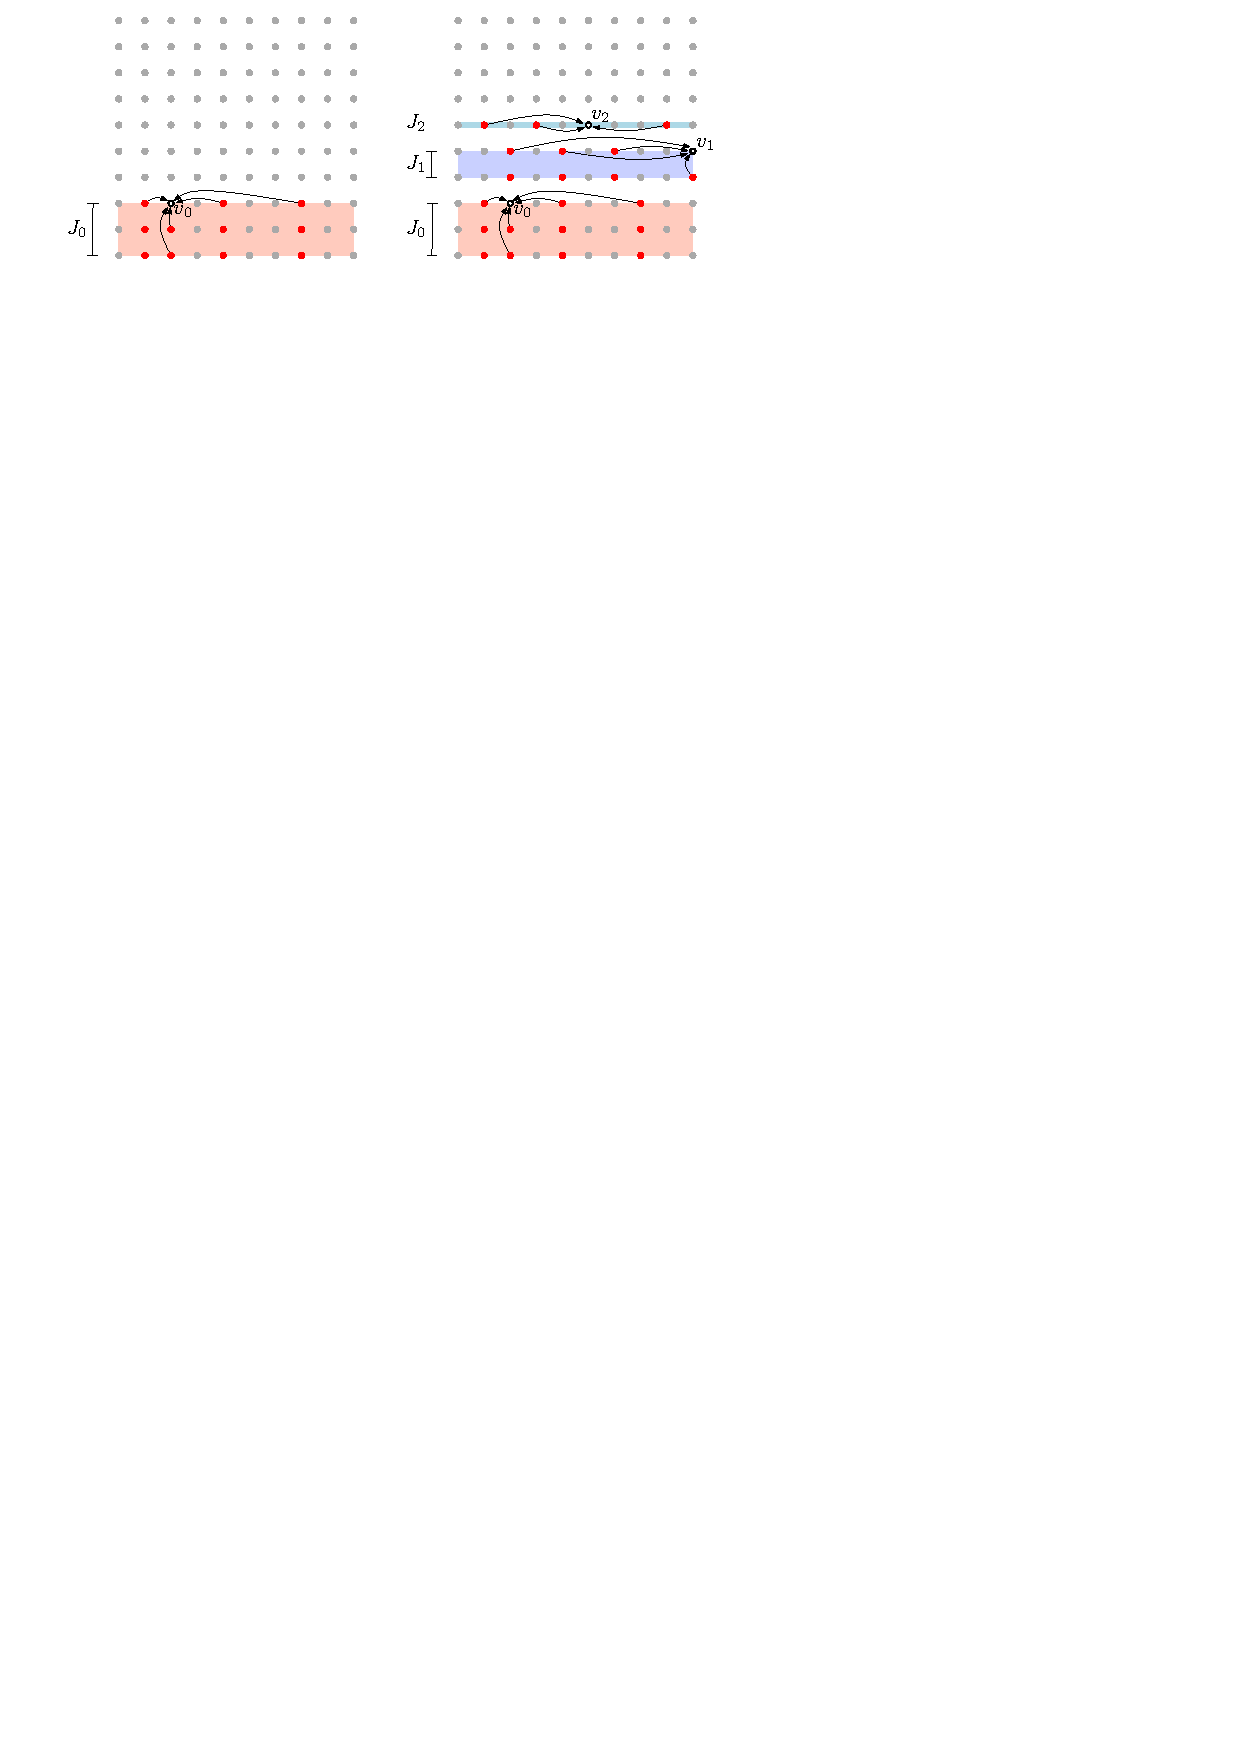
\includegraphics[width=1\textwidth]{ClimbingLemma.pdf}
\caption{\small Illustration for the first part of the proof of Lemma~\ref{lemma:Climbing lemma}.}
\label{fig:Climbing Lemma}
\end{figure}

Since $0 < \beta < 1$, after $k = O(1)$ iterations, the above procedure stops. 
Because the process stopped, we know that $|B_{k+1}| = |B_k \setminus J_{v_k}| <  \frac{n}{2}$.
Since $B_{k+1} = B_0\setminus \cup_{i=0}^k J_{v_i}$, we know that $|\cup_{i=0}^k J_{v_i}| >  \frac{n}{2}$.

Compute an $s \in \join(\{v_0, \ldots, v_k\})$ and notice that $s$ is smaller than $v_i$ for each $1\leq i\leq k$. Since $k = O(1)$, $s$ can be computed using $O(1)$ vertex queries. 
Assume that $s = (x_s, y_s)$ and let $s'$ be the sink of the $\{x_s\}\times \cup_{i=0}^k J_{v_i}$-subgrid. 
Let $0\leq h\leq k$ be an integer such that $s'$ belongs to the $[m]\times J_{v_h}$-subgrid; see Figure~\ref{fig:Climbing Lemma-2}.

\begin{figure}[h]
\centering
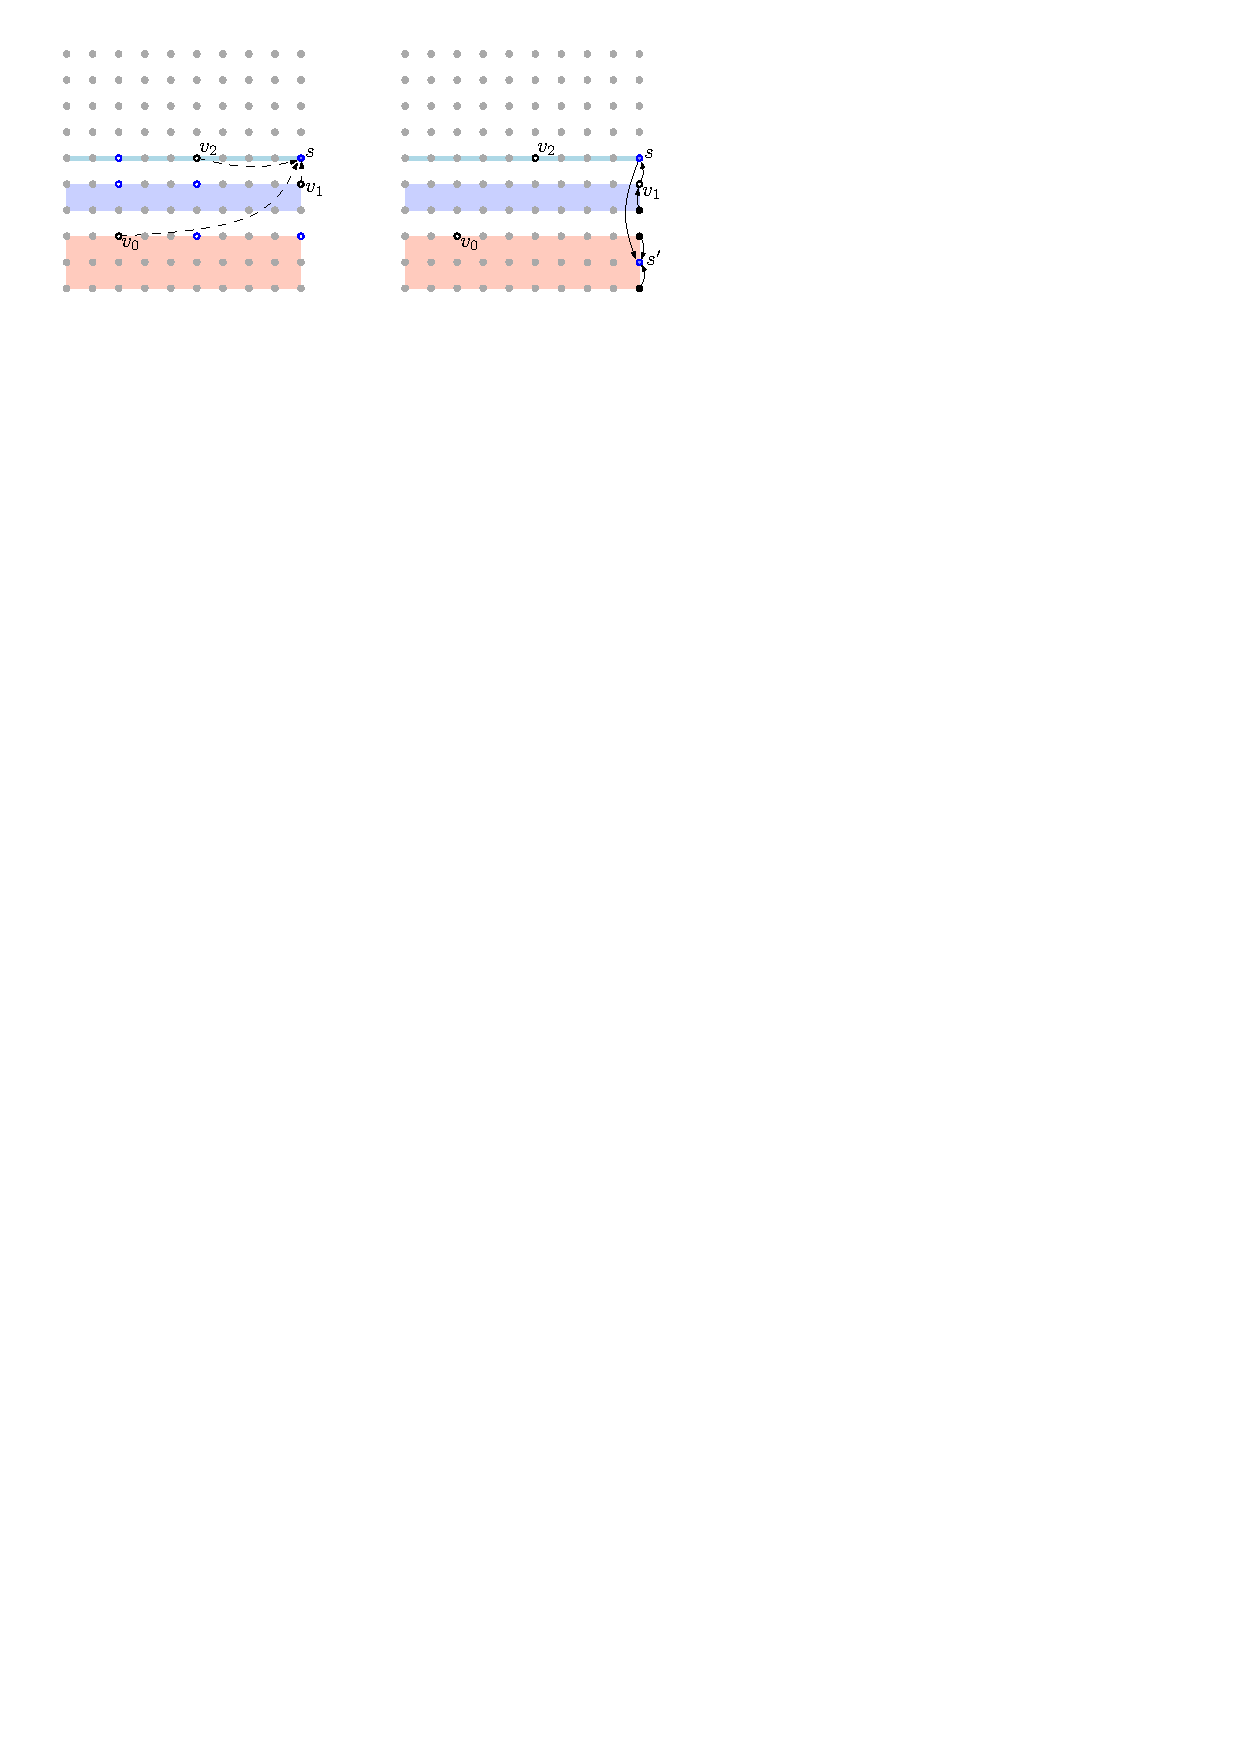
\includegraphics[width=0.85\textwidth]{ClimbingLemma-2.pdf}
\caption{\small Illustration for the latter part of the proof of Lemma~\ref{lemma:Climbing lemma}.}
\label{fig:Climbing Lemma-2}
\end{figure}

Let $[a,b]$ be the \indegree of $s'$.
Recall that $s$ is smaller than $v_h$, hence $s'$ is also smaller than $v_h$.
Because $v_h$ is the sink of the $I_{v_h}\times J_{v_h}$-grid, $s'$ is smaller than each vertex in the $I_{v_h}\times J_{v_h}$-grid.
Therefore, at least $|I_{v_h}|$ vertices have outgoing edges to $s'$ in the row containing $s'$, i.e., $a\geq |I_{v_h}| \geq \alpha m$.
Moreover, since $s'$ is the sink of the $\{x_s\}\times \cup_{i=0}^k J_{v_i}$-subgrid, $b \geq |\cup_{i=0}^k J_{v_i}|  >  \frac{n}{2}$.
Consequently, $s'$ is an $(\alpha m,  \frac{n}{2})$-vertex. \qed
\end{proof}

The above lemma can be generalized to the following corollary, which we state without proof. 
\begin{corollary}\label{corollary: (m/2,n/2) indegree}
Let $G$ be an $(m,n)$-grid USO. 
We can compute an $( \frac{m}{2}, \frac{n}{2})$-vertex using $O(m + n)$ vertex queries.
\end{corollary}

Our main result can now be proved by combining the Lemmas and Corollaries we established in this section. 

\begin{theorem}\label{theorem:Sink algorithm}
The sink of an $(m,n)$-grid USO can be found with \\ $O((m+n)\log (m+n))$ vertex queries.
\end{theorem}

\section{The Edge Oracle Model}
\label{section:The edge oracle model}

In the previous sections we have mainly discussed the vertex oracle model.
In the \emph{edge oracle model} considered here, the algorithm accesses the
grid by means of an \emph{edge oracle} which can tell us
the orientation of any given edge.
One can show by an adversary argument that $\Omega(m+n)$ queries are necessary in the worst case.
An easy upper bound is $O(mn)$ (find the sink of each row individually; then
for each of these local sinks, query all incident edges to decide whether it
is the global sink).
But we can do better:

\begin{theorem}
    \label{thm:timeEdge}
    To find the sink in an $(m,n)$-grid USO with a deterministic algorithm,
    $O((m+n) ^ {\log_4(7)})$ edge queries suffice; $\log_4(7) \approx
    1.40$.
\end{theorem}

To proof of Theorem~\ref{thm:timeEdge} uses the following result for the \emph{vertex} oracle model.

\begin{lemma}
    \label{lem:4:7}
    There is a deterministic algorithm which finds the sink in a
    $(4,4)$-grid USO and which uses at most 7 vertex queries.
\end{lemma}

\MM{Improve this sentence}
For the proof of the lemma we refer the reader to the full version of this paper, where we describe how we reduce the problem to three cases, using a computer search to eliminate symmetrical situations. 

\begin{proof}[of Theorem~\ref{thm:timeEdge}]
    Let $N = m+n$.
    We describe a sink-finding algorithm which uses
    $T(N) \in O(N ^ {\log_4(7)})$ edge queries.
    Without loss of generality, we will assume that $m$ is a power of $4$, and
    $m=n$. Otherwise, we can satisfy this property with adding at most linearly many rows and columns while maintaining the position of the sink.

    Given an $(m,m)$-grid $G$, let $\A$
    be a partition of the index set $[m]$ such that
    $|\A| = 4$ and $|A| = \frac{m}{4}$ for all $A \in \A$.
    Consider the induced unique sink orientation on the \aapart $H$.
    
    
    Let $v$ be a vertex of $H$. Recall that $v$ corresponds to an $(\frac{m}{4},\frac{m}{4})$-subgrid of $G$.
    We can find the sink $s_v$ of the subgrid $v$ using a recursive call that takes $T(N/4)$ edge queries.
    Afterwards we can find out the orientations of the six edges
    adjacent to the vertex $v$ in $H$ by querying the $N-2$ edges adjacent to $s_v$ in $G$.
    Thus we have simulated a vertex query in $H$ using at most $T(N/4) + N$ edge queries in $G$.

    Now, using Lemma~\ref{lem:4:7} to tell us \emph{which} vertex
    queries to simulate, we will find the sink of $H$
    % $\sink(G) = \sink(G(\sink(H)))$ (see~Lemma
    %\ref{lemma:USO-Lemma})
    after at most
    \[
        T(N) \le 7 \cdot \Bigl( T \left( N/4 \right) + N \Bigr)
    \]
    edge queries in $G$ and therefore $T(N) \in O(N ^ {\log_4(7)})$. 
    Recall that algorithm from Lemma~\ref{lem:4:7} also queries the sink $s_H$ of $H$, and by Lemma~\ref{lemma:USO-Lemma} the sink $s_G$ of $G$ equals the sink of the subgrid $s_H$. Therefore we have in the process also found and queried the edges adjacent to $s_G$.
    \qed
\end{proof}

\bibliographystyle{abbrvnat}
\bibliography{griduso}

\end{document}
